% chktex-file 2% chktex-file 29
% chktex-file 13
\documentclass{report}
\usepackage{setspace}
\usepackage[a4paper, total={7in, 10in}]{geometry}
\usepackage[fleqn]{amsmath}
\usepackage{empheq}
\usepackage{amssymb}
\usepackage{amsthm}
\usepackage{gensymb}
\usepackage[fleqn]{cases}
\usepackage{multicol}
\usepackage{color}
\usepackage{stix}
\usepackage{chngcntr}
\usepackage{tikz}
\usepackage{enumitem}
\usepackage{pgfplots}
\usepackage{etoolbox}
\usepackage{tikz-3dplot}
\usepackage{tkz-euclide}
\usepackage{graphicx}
\graphicspath{ {./assets/} }
\usetikzlibrary{calc,matrix,arrows}
\usetikzlibrary{decorations.pathmorphing,patterns, calligraphy, perspective,backgrounds}

\tikzset{
    right angle quadrant/.code={
            \pgfmathsetmacro\quadranta{{1,1,-1,-1}[#1-1]}     % Arrays for selecting quadrant
            \pgfmathsetmacro\quadrantb{{1,-1,-1,1}[#1-1]}},
    right angle quadrant=1, % Make sure it is set, even if not called explicitly
    right angle length/.code={\def\rightanglelength{#1}},   % Length of symbol
    right angle length=2ex, % Make sure it is set...
    right angle symbol/.style n args={3}{
            insert path={
                    let \p0 = ($(#1)!(#3)!(#2)$) in     % Intersection
                    let \p1 = ($(\p0)!\quadranta*\rightanglelength!(#3)$), % Point on base line
                    \p2 = ($(\p0)!\quadrantb*\rightanglelength!(#2)$) in % Point on perpendicular line
                    let \p3 = ($(\p1)+(\p2)-(\p0)$) in  % Corner point of symbol
                    (\p1) -- (\p3) -- (\p2)
                }
        }
}

\counterwithout{equation}{chapter}
\setlength{\columnseprule}{1pt}
\setlength{\columnsep}{24pt}
\setcounter{chapter}{14}
\hfuzz=100pt

\newcommand{\pgfplotsdrawaxis}{\pgfplots@draw@axis}
\makeatother
\pgfplotsset{only axis on top/.style={axis on top=false, after end axis/.code={
                    \pgfplotsset{axis line style=opaque, ticklabel style=opaque, tick style={thick,opaque},
                        grid=none}\pgfplotsdrawaxis}}}

\newtheorem{theorem}{Theorem}

\begin{document}

\newcommand{\planelineinter}[5]% a, b, c, p as {a_x,a_y,a_z}, coordinate name
{   \foreach \a [count=\k] in {#1}
        { \ifthenelse{\k=1}{\xdef\tempxa{\a}}
            \ifthenelse{\k=2}{\xdef\tempya{\a}}
            \ifthenelse{\k=3}{\xdef\tempza{\a}}
        }
    \foreach \b [count=\k] in {#2}
        { \ifthenelse{\k=1}{\xdef\tempxb{\b}}
            \ifthenelse{\k=2}{\xdef\tempyb{\b}}
            \ifthenelse{\k=3}{\xdef\tempzb{\b}}
        }
    \foreach \c [count=\k] in {#3}
        { \ifthenelse{\k=1}{\xdef\tempxc{\c}}
            \ifthenelse{\k=2}{\xdef\tempyc{\c}}
            \ifthenelse{\k=3}{\xdef\tempzc{\c}}
        }
    \foreach \p [count=\k] in {#4}
        { \ifthenelse{\k=1}{\xdef\tempxp{\p}}
            \ifthenelse{\k=2}{\xdef\tempyp{\p}}
            \ifthenelse{\k=3}{\xdef\tempzp{\p}}
        }
    \pgfmathsetmacro{\abx}{\tempxb-\tempxa}
    \pgfmathsetmacro{\aby}{\tempyb-\tempya}
    \pgfmathsetmacro{\abz}{\tempzb-\tempza}
    \pgfmathsetmacro{\acx}{\tempxc-\tempxa}
    \pgfmathsetmacro{\acy}{\tempyc-\tempya}
    \pgfmathsetmacro{\acz}{\tempzc-\tempza}
    \pgfmathsetmacro{\nx}{\aby*\acz-\abz*\acy}
    \pgfmathsetmacro{\ny}{\abz*\acx-\abx*\acz}
    \pgfmathsetmacro{\nz}{\abx*\acy-\aby*\acx}
    \pgfmathsetmacro{\d}{(\nx+\ny+\nz)/(\nx*\tempxp+\ny*\tempyp+\nz*\tempzp)}
    \path (0,0,0) -- (#4) coordinate[pos=\d] (#5);
}

% golden ratio and inverse golden ratio
\pgfmathsetmacro{\gr}{(1+sqrt(5))/2}
\pgfmathsetmacro{\igr}{2/(1+sqrt(5))}

%choose axis angles
\newcommand{\xangle}{0}
\newcommand{\yangle}{90}
\newcommand{\zangle}{225}

%choose axis lengths
\newcommand{\xlength}{1}
\newcommand{\ylength}{1}
\newcommand{\zlength}{0.5}

\pgfmathsetmacro{\xx}{\xlength*cos(\xangle)}
\pgfmathsetmacro{\xy}{\xlength*sin(\xangle)}
\pgfmathsetmacro{\yx}{\ylength*cos(\yangle)}
\pgfmathsetmacro{\yy}{\ylength*sin(\yangle)}
\pgfmathsetmacro{\zx}{\zlength*cos(\zangle)}
\pgfmathsetmacro{\zy}{\zlength*sin(\zangle)}

\newcommand{\sol}[1]{

    \noindent \textbf{Sol.}
}
\newcommand{\prooff}[1]{

    \noindent \textbf{Proof.}
}
\newcommand\m[1]{\begin{pmatrix}#1\end{pmatrix}}
\newcommand\vm[1]{\begin{vmatrix}#1\end{vmatrix}}
\newenvironment{amatrix}[1]{%
    \left(\begin{array}{@{}*{#1}{c}|c@{}}
        }{%
    \end{array}\right)
}
\newenvironment{cequation}{
    \makeatletter
    \setbool{@fleqn}{false}
    \makeatother
    \begin{equation*}
        }{\end{equation*}}

\begin{titlepage}
    \raggedleft{}
    \rule{1pt}{\textheight}
    \hspace{0.02\textwidth}
    \parbox[b]{0.75\textwidth}{

    {\Huge\bfseries Solution Book of \\[0.5\baselineskip] Mathematic}\\[2\baselineskip]
    {\large\textit{Ssnior 2 Part I}}\\[4\baselineskip]
    {\Large\textsc{MELVIN CHIA}}

    \vspace{0.5\textheight}

    {\noindent Written on 9 October 2022}\\[\baselineskip]
    }

\end{titlepage}

\doublespacing{}
\tableofcontents
\singlespacing{}
\newpage

\begin{multicols}{2}

    \chapter{Solid Geometry, Longitude and Latitude}

    \section{Solid Geometry}

    \subsection*{Polyhedron}

    A polyhedron is a solid bounded by a finite amount of flat polygon, and each
    side of the polygons must be the common edge of two polygons. Polyhedron can be
    classified into tetrahedron, pentahedron, hexahedron, etc. based on the number
    of flat surfaces, aka the \emph{faces} of the polyhedron. The common side of
    two faces of a polyhedron is called an edge, and the common vertex of three
    edges is called an \emph{apex}.

    Besides, the angles formed by the faces intersecting at the same apex are
    called \emph{polyhedral angles} or \emph{solid angles}. The line segment
    connecting two apexes at different faces is called a \emph{diagonal}.

    \begin{center}
        \tdplotsetmaincoords{70}{70}
        \begin{tikzpicture}[scale=0.6,tdplot_main_coords,declare function={d=6;}]
            \path (0,0,0)       coordinate (A)
            (d/2,d/2,0)     coordinate (H)
            (d,0,0)        coordinate (C)
            (d/2,{d*sqrt(3)/2},0)    coordinate (B)
            (d/2,d/2,{d/sqrt(2)}) coordinate (D)
            ($ (A)!0.5!(C) $) coordinate (M);
            \foreach \p/\g in {A/-90,B/-90,C/-90,D/90}
            \path (\p)+(\g:3mm);
            \draw (D) -- (A) (D) -- (B) (D) -- (C) (A) -- (C) -- (B);
            \draw [dashed] (A) -- (B);
            \node at (C) [below=10pt] {Tetrahedron};
        \end{tikzpicture}
        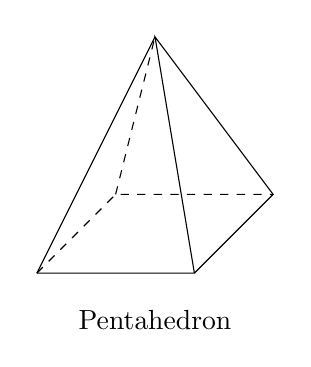
\begin{tikzpicture}
            \tikzstyle{point}=[circle,thick,draw=black,fill=black,inner sep=0pt,minimum width=4pt,minimum height=4pt]
            \node (a) at (0,0) {};
            \node (b) at (2,0) {};
            \node (c) at (3,1) {};
            \node (d) at (1,1) {};
            \node (e) at (1.5,3) {};
            \draw (a.center) -- (b.center) -- (c.center) -- (e.center) -- (b.center);
            \draw (a.center) -- (e.center);
            \draw[dashed] (a.center) -- (d.center) -- (c.center);
            \draw[dashed] (d.center) -- (e.center);
            \node at (1.5,0) [below=10pt] {Pentahedron};
        \end{tikzpicture}
    \end{center}
    \begin{center}
        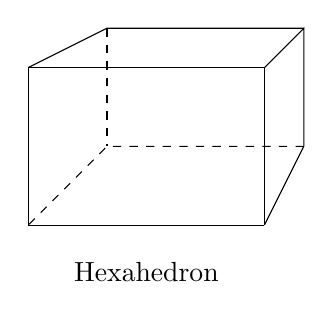
\begin{tikzpicture}
            \draw (0,0)--(3,0);
            \draw (3,0)--(3.5,1);
            \draw[dashed] (3.5,1)--(1,1)--(0,0);
            \draw (0,0)--(0,2)--(3,2)--(3,0);
            \draw (0,2)--(1,2.5)--(3.5,2.5);
            \draw[] (3,2)--(3.5,2.5)--(3.5,1);
            \draw[dashed] (1,2.5)--(1,1);
            \node at (1.5,0) [below=10pt] {Hexahedron};
        \end{tikzpicture}
    \end{center}

    \subsection*{Regular Polyhedron}

    A \emph{regular polyhedron} is a polyhedron with all faces being regular
    polygons, and all polyhedral angles being equal. The regular polyhedron can be
    classified into 5 types: \emph{regular tetrahedron}, \emph{regular octahedron},
    \emph{regular hexahedron}, \emph{regular dodecahedron} and \emph{regular
        icosahedron}.

    \begin{center}
        \tdplotsetmaincoords{70}{100}
        \begin{tikzpicture}[scale=0.7,line join=round,tdplot_main_coords,declare function={a=5;}]
            \begin{scope}[canvas is xy plane at z=0,transform shape]
                \path foreach \X [count=\Y] in {A,B,C}
                    {(\Y*120:{a/(2*cos(30))}) coordinate(\X)};
            \end{scope}
            \path (0,0,{a*cos(30)}) coordinate (D);
            \draw [dashed] (A) -- (D) -- (B) -- (A);
            \draw (B) -- (D) -- (C) -- (B);
            \draw (C) -- (D) -- (A) -- (C);
            \node at (0,0,0) [below=30pt] {Regular Tetrahedron};
        \end{tikzpicture}
        \hspace*{1cm}
        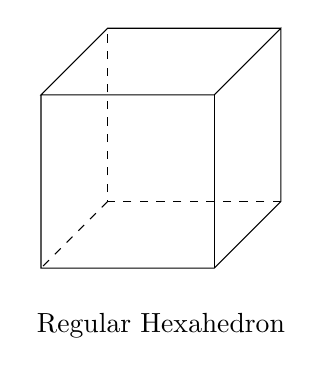
\begin{tikzpicture}[scale=1.1]
            \draw (2,2,0)--(0,2,0)--(0,2,2)--(2,2,2)--(2,2,0)--(2,0,0)--(2,0,2)--(0,0,2)--(0,2,2);
            \draw (2,2,2)--(2,0,2);
            \draw[dashed](2,0,0)--(0,0,0)--(0,2,0);
            \draw[dashed](0,0,0)--(0,0,2);
            \node at (1,1,1) [below=56pt] {Regular Hexahedron};
        \end{tikzpicture}
    \end{center}

    \begin{center}
        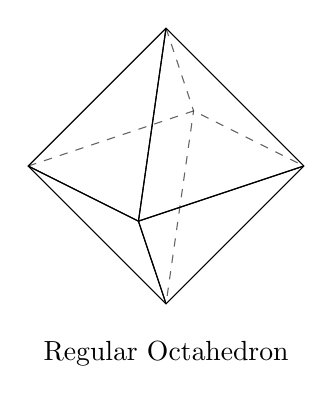
\begin{tikzpicture}[scale=3.5]

            \coordinate (A1) at (0,0);
            \coordinate (A2) at (0.6,0.2);
            \coordinate (A3) at (1,0);
            \coordinate (A4) at (0.4,-0.2);
            \coordinate (B1) at (0.5,0.5);
            \coordinate (B2) at (0.5,-0.5);

            \begin{scope}[dashed,opacity=0.6]
                \draw (A1) -- (A2) -- (A3);
                \draw (B1) -- (A2) -- (B2);
            \end{scope}
            \draw (A1) -- (A4) -- (B1);
            \draw (A1) -- (A4) -- (B2);
            \draw (A3) -- (A4) -- (B1);
            \draw (A3) -- (A4) -- (B2);
            \draw (B1) -- (A1) -- (B2) -- (A3) --cycle;
            \node at (0.5,-0.5) [below=10pt] {Regular Octahedron};
        \end{tikzpicture}
        \hspace*{1cm}
        \begin{tikzpicture}[scale=1]
            [   x={(\xx cm,\xy cm)},
                y={(\yx cm,\yy cm)},
                z={(\zx cm,\zy cm)},
                scale=2,
            ]

            % vertices of inscribed cube
            \coordinate (pd1) at (-1,-1,-1);
            \coordinate (pd2) at (-1,-1,1);
            \coordinate (pd3) at (-1,1,-1);
            \coordinate (pd4) at (-1,1,1);
            \coordinate (pd5) at (1,-1,-1);
            \coordinate (pd6) at (1,-1,1);
            \coordinate (pd7) at (1,1,-1);
            \coordinate (pd8) at (1,1,1);
            % "front/back" "outside of cube" points
            \coordinate (pd9) at (0,-\igr,-\gr);
            \coordinate (pd10) at (0,-\igr,\gr);
            \coordinate (pd11) at (0,\igr,-\gr);
            \coordinate (pd12) at (0,\igr,\gr);
            % "top/bottom" "outside of cube" points
            \coordinate (pd13) at (-\igr,-\gr,0);
            \coordinate (pd14) at (-\igr,\gr,0);
            \coordinate (pd15) at (\igr,-\gr,0);
            \coordinate (pd16) at (\igr,\gr,0);
            % "left/right" "outside of cube" points
            \coordinate (pd17) at (-\gr,0,-\igr);
            \coordinate (pd18) at (-\gr,0,\igr);
            \coordinate (pd19) at (\gr,0,-\igr);
            \coordinate (pd20) at (\gr,0,\igr);

            % edges on "back"    face of inscribes cube; red
            \draw[dashed] (pd9) -- (pd11);
            \draw[dashed] (pd11) -- (pd3);
            \draw[dashed] (pd11) -- (pd7);
            \draw[dashed] (pd9) -- (pd1);
            \draw[dashed] (pd9) -- (pd5);
            % edges on "top"     face of inscribes cube
            \draw[] (pd14) -- (pd16);
            \draw[] (pd16) -- (pd8);
            \draw[] (pd16) -- (pd7);
            \draw[dashed] (pd14) -- (pd3);
            \draw[] (pd14) -- (pd4);
            % edges on "left"    face of inscribes cube
            \draw[dashed] (pd17) -- (pd18);
            \draw[dashed] (pd17) -- (pd3);
            \draw[dashed] (pd17) -- (pd1);
            \draw[] (pd18) -- (pd2);
            \draw[] (pd18) -- (pd4);
            % edges on "bottom"  face of inscribes cube
            \draw[] (pd13) -- (pd15);
            \draw[dashed] (pd13) -- (pd1);
            \draw[] (pd13) -- (pd2);
            \draw[] (pd15) -- (pd5);
            \draw[] (pd15) -- (pd6);
            % edges on "front"   face of inscribes cube
            \draw[] (pd10) -- (pd12);
            \draw[] (pd12) -- (pd4);
            \draw[] (pd12) -- (pd8);
            \draw[] (pd10) -- (pd2);
            \draw[] (pd10) -- (pd6);
            % edges on "right"   face of inscribes cube 
            \draw[] (pd20) -- (pd19);
            \draw[] (pd19) -- (pd7);
            \draw[] (pd19) -- (pd5);
            \draw[] (pd20) -- (pd8);
            \draw[] (pd20) -- (pd6);

            \node at (0,-2.4,0) {Regular Dodecahedron};
        \end{tikzpicture}
    \end{center}
    \begin{center}
        \def \phi {1.617}
        \begin{tikzpicture}[
                x={(-0.86in, -0.5in)}, y = {(0.86in, -0.5in)}, z = {(0, 1in)},
                rotate = 22,
                scale = 0.2,
                foreground/.style = {  },
                background/.style = { dashed }
            ]
            \coordinate (9) at (0, -\phi*\phi,  \phi);
            \coordinate (8) at (0,  \phi*\phi,  \phi);
            \coordinate (12) at (0,  \phi*\phi, -\phi);
            \coordinate (5) at (0, -\phi*\phi, -\phi);
            \coordinate (7) at ( \phi, 0,  \phi*\phi);
            \coordinate (3) at (-\phi, 0,  \phi*\phi);
            \coordinate (6) at (-\phi, 0, -\phi*\phi);
            \coordinate (4) at ( \phi, 0, -\phi*\phi);
            \coordinate (2) at ( \phi*\phi,  \phi, 0);
            \coordinate (10) at (-\phi*\phi,  \phi, 0);
            \coordinate (1) at (-\phi*\phi, -\phi, 0);
            \coordinate (11) at ( \phi*\phi, -\phi, 0);

            \draw[foreground] (10) -- (3) -- (8) -- (10) -- (12) -- (8);
            \draw[foreground] (4) -- (12) -- (2) -- (4) -- (11) -- (2);
            \draw[foreground] (9) -- (3) -- (7) -- (9) -- (11) -- (7);
            \draw[foreground] (7) -- (8) -- (2) -- cycle;
            \draw[background] (12) -- (6) -- (10) -- (1) -- (6) -- (5) -- (1)
            -- (9) -- (5) -- (11);
            \draw[background] (5) -- (4) -- (6);
            \draw[background] (3) -- (1);

            \node at (6,3.8,0) {Regular Icosahedron};
        \end{tikzpicture}
    \end{center}

    \subsection*{Prism}

    If two faces of a polyhedron are parallel, while the other faces intersect in
    sequence to form parallel lines, then the polyhedron is called a \emph{prism}.
    The two faces which are parallel to each other are called the \emph{bases of
        the prism}, and the other faces are called the \emph{lateral faces of the
        prism}. The common sides that two adjacent lateral faces share is called the
    \emph{lateral edges of the prism}. The distance between two bases is called the
    \emph{height of the prism}.

    Prism with lateral edges that aren't parallel to each other are called
    \emph{oblique prism}; prism with lateral edges that are parallel to each other
    are called \emph{right prism}; regular prism with regular bases are called
    \emph{regular prism}.

    \begin{center}
        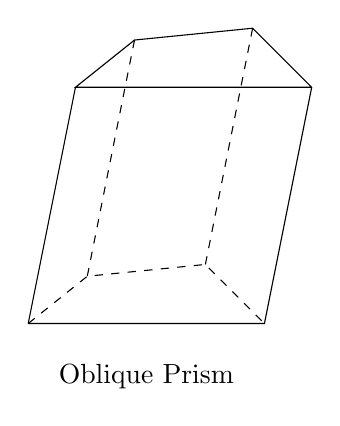
\begin{tikzpicture}[scale=1.5]
            \draw  [dashed] (-1,0) -- (-0.5,0.4) -- (0.5,0.5) edge (0.9,2.5) -- (1,0);
            \draw [dashed] (-0.1, 2.4) -- (-0.5,0.4);
            \draw (-1,0) -- (1, 0) -- (1.4, 2) -- (0.9,2.5) -- (-0.1, 2.4) -- (-0.6,2) -- (1.4, 2);
            \draw (-0.6, 2) -- (-1, 0);
            \node at (0,-0.45) {Oblique Prism};
        \end{tikzpicture}
        \hspace*{1cm}
        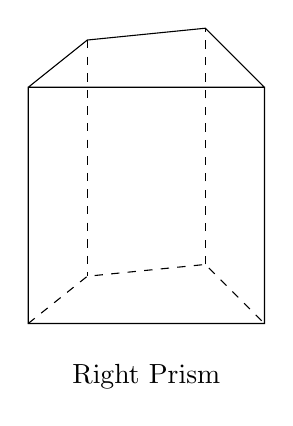
\begin{tikzpicture}[scale=1.5]
            \draw[dashed] (-1,0) -- (-0.5,0.4) -- (0.5,0.5) edge (0.5,2.5) -- (1,0);
            \draw [dashed] (-0.5, 2.4) -- (-0.5,0.4);
            \draw (-1,0)  rectangle (1,2) -- (0.5,2.5) -- (-0.5, 2.4) -- (-1,2);
            \node at (0,-0.45) {Right Prism};
        \end{tikzpicture}

    \end{center}
    \begin{center}
        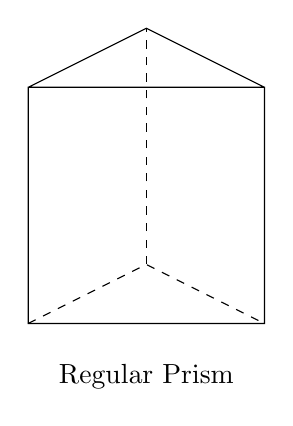
\begin{tikzpicture}[scale=1.5]
            \draw[dashed] (-1,0) -- (0,0.5) edge (0,2.5) -- (1,0) coordinate(BR);
            \draw (-1,0) coordinate(BL)  rectangle (1,2) coordinate(TR)
            -- (0,2.5) coordinate(T) -- (-1,2) coordinate(TL);
            \node at (0,-0.45) {Regular Prism};
        \end{tikzpicture}
    \end{center}

    Prism with bases of parallelogram are called \emph{parallelepiped}.
    Parallelepiped with lateral edges that are parallel to each other are called
    \emph{right parallelepiped}. Right parallelepiped with regular bases are called
    \emph{cuboid}, and a cuboid with equal width, height, and depth is called a
    \emph{cube}.

    \begin{center}
        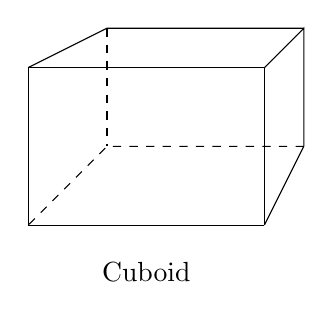
\begin{tikzpicture}
            \draw (0,0)--(3,0);
            \draw (3,0)--(3.5,1);
            \draw[dashed] (3.5,1)--(1,1)--(0,0);
            \draw (0,0)--(0,2)--(3,2)--(3,0);
            \draw (0,2)--(1,2.5)--(3.5,2.5);
            \draw[] (3,2)--(3.5,2.5)--(3.5,1);
            \draw[dashed] (1,2.5)--(1,1);
            \node at (1.5,0) [below=10pt] {Cuboid};
        \end{tikzpicture}
        \hspace*{1cm}
        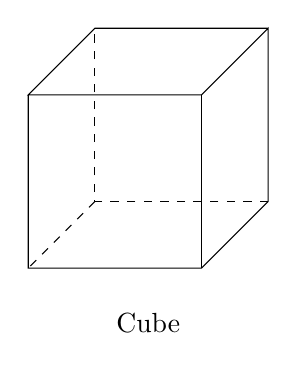
\begin{tikzpicture}[scale=1.1]
            \draw (2,2,0)--(0,2,0)--(0,2,2)--(2,2,2)--(2,2,0)--(2,0,0)--(2,0,2)--(0,0,2)--(0,2,2);
            \draw (2,2,2)--(2,0,2);
            \draw[dashed](2,0,0)--(0,0,0)--(0,2,0);
            \draw[dashed](0,0,0)--(0,0,2);
            \node at (1,1,1) [below=56pt] {Cube};
        \end{tikzpicture}
    \end{center}

    \subsection*{Pyramid}

    If a polyhedron has a polygonal base and all its lateral faces are triangles
    that shares a common apex, then the polyhedron is called a \emph{pyramid}.

    If the foot point of a pyramid is the centre of its base, then the pyramid is
    called a \emph{right pyramid}. If the base of a right pyramid is a regular
    polygon, then the pyramid is called a \emph{regular pyramid}.

    \begin{center}
        \tdplotsetmaincoords{70}{120}
        \begin{tikzpicture}[scale=0.7,tdplot_main_coords,line cap=butt,line join=round,c/.style={circle,fill,inner sep=1pt},
                declare function={a=4;h=3;}]
            \path
            (0,0,0) coordinate (A)
            (a,0,0) coordinate (B)
            (a+2,a+2,0) coordinate (C)
            (0,a,0) coordinate (D)
            (a/2 + 1,a/2 + 1,0) coordinate (O)
            (a/2 + 1,a/2 + 1,h)  coordinate (S);
            \draw (S) -- (D) -- (C) -- (B) -- cycle (S) -- (C);
            \draw[dashed] (S) -- (A) --(D) (A) -- (B) ;

            \node at (a/2 + 1,a/2+0.5,0) [below=40pt] {Right Pyramid};
        \end{tikzpicture}
        \hspace*{1cm}
        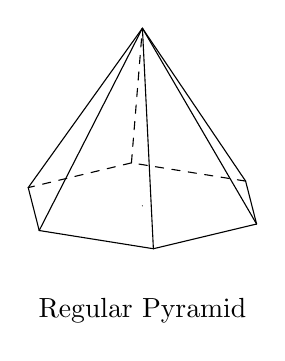
\begin{tikzpicture}[scale=0.8,3d view={55}{20},declare function={a=2;b=3;l=5;},
                >=stealth,line cap=round,line join=round]
            \draw  (tpp cs:x=0,y=0,z=0) coordinate (O) -- (O);
            \path foreach \X in {1,...,6}
            {(tpp cs:x={a*cos(\X*60-30)},y={a*sin(\X*60-30)},z=0) coordinate (p\X)}
            (tpp cs:x=0,y=0,z=b) coordinate (tip);
            \draw (p1) -- (p2);
            \draw [dashed] (p2) -- (p3);
            \draw [dashed] (p3) -- (p4);
            \draw (p4) -- (p5);
            \draw (p5) -- (p6);
            \draw (p6) -- (p1);
            \draw (p1) -- (tip);
            \draw (p2) -- (tip);
            \draw [dashed] (p3) -- (tip);
            \draw (p4) -- (tip);
            \draw (p5) -- (tip);
            \draw (p6) -- (tip);

            \node at (0,0,0) [below=30pt] {Regular Pyramid};
        \end{tikzpicture}
    \end{center}

    \subsection*{Right Circular Cylinder}

    A \emph{right circular cylinder} is the solid of revolution generated by
    rotating a rectangle about one of its sides.

    \begin{center}
        \def\myr{2}
        \def\h{5}
        \def\angA{0}
        \def\angB{60}
        \tdplotsetmaincoords{80}{60}
        \begin{tikzpicture}[tdplot_main_coords,scale=0.6]
            %    \draw[-latex] (0,0,0) -- (1,0,0) node[pos=1.1]{$x$};
            %    \draw[-latex] (0,0,0) -- (0,1,0) node[pos=1.1]{$y$};
            %    \draw[-latex] (0,0,0) -- (0,0,1) node[pos=1.1]{$z$};
            \begin{scope}[canvas is xy plane at z=0]
                \path (0,0) (O);
                \draw[dashed] (\tdplotmainphi:\myr) arc(\tdplotmainphi:\tdplotmainphi+180:\myr);
                \path (\angA:\myr) coordinate (A) -- (\angB:\myr) coordinate (B);
                \draw (\tdplotmainphi:\myr) coordinate(BR) arc(\tdplotmainphi:\tdplotmainphi-180:\myr)
                coordinate(BL);
            \end{scope}
            %
            \begin{scope}[canvas is xy plane at z=\h]
                \draw (0,0) coordinate (O') circle[radius=\myr];
                \path (\angA:\myr) coordinate (A') -- (\angB:\myr) coordinate (B');
                \draw (BR) -- (\tdplotmainphi:\myr) (BL) -- (\tdplotmainphi-180:\myr);
                \draw (B) -- (B');
            \end{scope}
        \end{tikzpicture}
    \end{center}

    \subsection*{Right Circular Cone}

    A \emph{right circular cone} is the solid of revolution generated by rotating a
    right-angled triangle about one of its sides.

    \begin{center}
        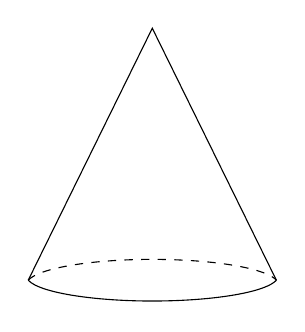
\begin{tikzpicture}[scale=0.8]
            \draw[dashed] (0,0) arc (170:10:2cm and 0.4cm)coordinate[pos=0] (a);
            \draw (0,0) arc (-170:-10:2cm and 0.4cm)coordinate (b);
            \draw (a) -- ([yshift=4cm]$(a)!0.5!(b)$) -- (b);
        \end{tikzpicture}
    \end{center}

    \subsection*{Sphere}

    The surface of revolution generated by rotating a semicircle about its diameter
    is called a \emph{spherical surface}, and the solid covered by it is called a
    \emph{sphere}.

    \begin{center}
        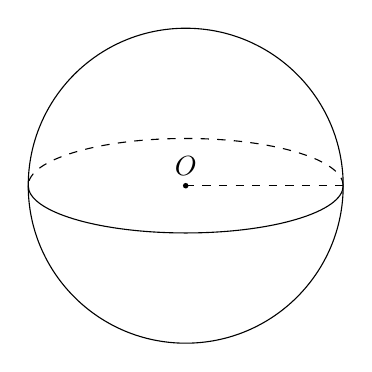
\begin{tikzpicture}
            \draw (0,0) circle (2cm);
            \draw (-2,0) arc (180:360:2 and 0.6);
            \draw[dashed] (2,0) arc (0:180:2 and 0.6);
            \fill[fill=black] (0,0) circle (1pt) node [above] {$O$};
            \draw[dashed] (0,0 ) -- (2,0);
        \end{tikzpicture}
    \end{center}

    If the circle is cut with a plane, the plane has the following properties:
    \begin{enumerate}
        \item The line joining the centre of the sphere to the centre of the plane are
              perpendicular to the plane.
        \item The distance of the plane from the centre of the sphere $d$, the radius of the
              sphere $R$ and the radius of the plane $r$ has the following relation:
              \begin{cequation}
                  r = \sqrt{R^2 - d^2}
              \end{cequation}
    \end{enumerate}

    \begin{center}
        \def\myangle{70}%
        \tdplotsetmaincoords{\myangle}{0}%
        \begin{tikzpicture}[scale=0.5,tdplot_main_coords]
            \pgfmathsetmacro{\r}{2*sqrt(3)}% sphere radius=4, cylendar height=4
            \path% common coordinates
            (0,0,-2) coordinate (O)
            (0,0,0) coordinate (I)
            (0,0,2) coordinate (O')
            (O) ++(0:\r) coordinate (C)% right edge
            (O) ++(180:\r) coordinate (D);% left edge
            \draw[dashed] (O)--(I) node [midway, left] {$d$};
            \begin{scope}[tdplot_screen_coords, on background layer]
                \draw (I) circle (4);
            \end{scope}

            \pgfmathsetmacro{\mynumer}{2*cos(\myangle)}
            \pgfmathsetmacro{\mydenom}{\r*sin(\myangle)}
            \pgfmathsetmacro{\quadrant}{ifthenelse(abs(\mynumer)<abs(\mydenom), 0,
                ifthenelse(\mynumer>0, 1, 2))}% 0=side, 1=top, 2=bottom

            \ifcase\quadrant
            \pgfmathsetmacro{\intercept}{asin(\mynumer/\mydenom)}
            \path
            (O) ++(-\intercept:\r) coordinate (A)
            (O) ++(-180+\intercept:\r) coordinate (B)
            (O') ++(\intercept:\r) coordinate (A')
            (O') ++(180-\intercept:\r) coordinate (B');
            \draw [thick] (B) arc (-180+\intercept:-\intercept:\r);
            \draw [thick, dashed] (A) arc (-\intercept:180+\intercept:\r);

            \draw[dashed] (O) --(A) node [midway, below] {$r$} (I) node [above] {$O$} --(A) node [midway, above] {$R$};
            \filldraw (I) circle (1.2pt);
            \tkzMarkRightAngle[size = 0.3](I,O,A);
        \end{tikzpicture}
    \end{center}

    The circle cut by a plane passing through the centre of the sphere is called a
    \emph{great circle}; the circle cut by a plane that does not pass through the
    centre of the sphere is called a \emph{small circle}.

    \section{Angles Formed by Planes and Straight Lines}

    There are three types of positional relationship between a plane and a straight
    line:

    \begin{enumerate}
        \item The line is on the plane
              \begin{center}
                  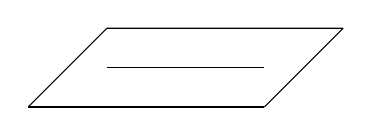
\begin{tikzpicture}
                      \draw (0,0)--(3,0);
                      \draw (3,0)--(4,1);
                      \draw (4,1)--(1,1)--(0,0);
                      \draw (1, 0.5) -- (3, 0.5);
                  \end{tikzpicture}
              \end{center}
        \item The line only intersects the plane at one point
              \begin{center}
                  \begin{tikzpicture}
                      \draw (0,0)--(3,0);
                      \draw (3,0)--(4,1);
                      \draw (4,1)--(1,1)--(0,0);
                      \draw (1.5, 2) -- (2, 0.5);
                      \draw [dashed] (2, 0.5) -- (2.5, -1);
                      \filldraw (2, 0.5) circle (1pt);
                  \end{tikzpicture}
              \end{center}
        \item The line does not intersect the plane
              \begin{center}
                  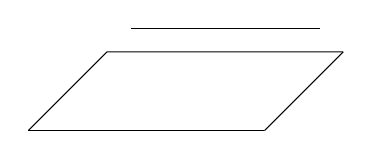
\begin{tikzpicture}
                      \draw (0,0)--(3,0);
                      \draw (3,0)--(4,1);
                      \draw (4,1)--(1,1)--(0,0);
                      \draw (1.3, 1.3) -- (3.7, 1.3);
                  \end{tikzpicture}
              \end{center}
    \end{enumerate}

    The angle formed by a line and the orthoprojection of the line on the plane is
    called \emph{the angle formed by the line and the plane}. This angle represents
    the inclination of the line with respect to the plane, thus it is called
    \emph{the tilt angle of the line with respect to the plane}.

    \subsection{Practice 1}

    \begin{enumerate}
        \item In the diagram below, $AB = 9cm$, $BC = 7cm$, $CG = 5cm$. Find:
              \begin{enumerate}
                  \item The angle formed by line $CF$ and plane $GHDC$.
                  \item The angle formed by line $DF$ and plane $EFGH$.
              \end{enumerate}
              \begin{center}
                  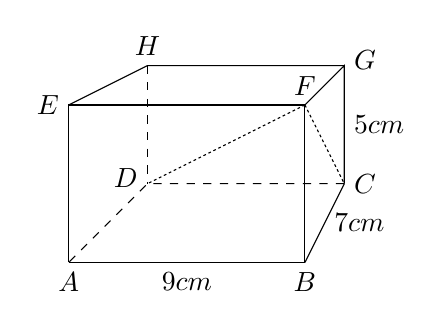
\begin{tikzpicture}
                      \draw (0,0) node [below] {$A$} --(3,0) node [below] {$B$} node[midway, below] {$9cm$};
                      \draw (3,0)--(3.5,1) node [right] {$C$} node [midway, right] {$7cm$};
                      \draw[dashed] (3.5,1)--(1,1) node [above=2pt, left] {$D$} --(0,0);
                      \draw (0,0)--(0,2) node[left] {$E$}--(3,2) node[above] {$F$} --(3,0);
                      \draw (0,2)--(1,2.5)--(3.5,2.5) node[above=2pt, right] {$G$};
                      \draw (3,2)--(3.5,2.5)--(3.5,1) node [midway, right] {$5cm$};
                      \draw[dashed] (1,2.5) node [above] {$H$} --(1,1);
                      \draw[dash pattern=on 1pt off 1pt] (3,2) -- (1,1);
                      \draw[dash pattern=on 1pt off 1pt] (3,2) -- (3.5,1);
                  \end{tikzpicture}
              \end{center}
        \item The diagram below shows a right prism, its base $KQL$ is a right-angled
              triangle, $JKLM$ is a square. Given that $JK = 12cm$, $LQ = 5cm$, find the
              angle formed by line $JQ$ and plane $PQLM$.
              \begin{center}
                  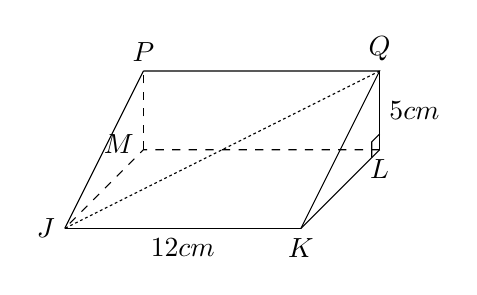
\begin{tikzpicture}
                      \draw (0,0) node [left] {$J$} --(3,0) node [below] {$K$} node [midway, below] {$12cm$};
                      \draw (3,0)--(4,1) node [below] {$L$};
                      \draw [dashed] (4,1)--(1,1) node [above=2pt, left] {$M$}--(0,0);
                      \draw [dashed] (1,1) -- (1,2) node [above] {$P$};
                      \draw (1,2)--(4,2) node [above] {$Q$} --(3,0);
                      \draw (4,2) -- (4,1) node [midway, right] {$5cm$};
                      \draw (1,2) -- (0,0);
                      \draw[dash pattern=on 1pt off 1pt] (4,2) -- (0,0);
                      \draw (4, 1.2) -- (3.9, 1.1) -- (3.9, 0.9);
                  \end{tikzpicture}
              \end{center}
    \end{enumerate}

    \subsection{Exercise 17.2}

    \begin{enumerate}
        \item The diagram below shows a cube with side length of $8.5cm$. Find:
              \begin{enumerate}
                  \item The angle formed by line $QS$ and plane $MNRQ$.
                  \item The angle formed by line $KQ$ and plane $PQML$.
              \end{enumerate}
              \begin{center}
                  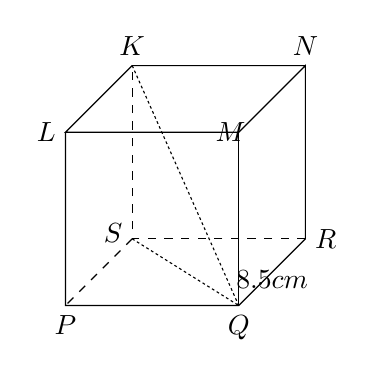
\begin{tikzpicture}[scale=1.1]
                      \draw (2,2,0) node [above] {$N$} --(0,2,0) node [above] {$K$} --(0,2,2) node [left] {$L$} --(2,2,2) node [above=6pt, left=-6pt] {$M$} --(2,2,0)--(2,0,0) node [right] {$R$}--(2,0,2)node [below] {$Q$} node [midway, right=16pt, below=-4pt] {$8.5cm$}--(0,0,2) node [below] {$P$}--(0,2,2);
                      \draw (2,2,2)--(2,0,2);
                      \draw[dashed](2,0,0)--(0,0,0)node [above=2pt, left] {$S$}--(0,2,0);
                      \draw[dashed](0,0,0)--(0,0,2);
                      \draw[dash pattern=on 1pt off 1pt] (0, 0, 0) -- (2,0,2);
                      \draw[dash pattern=on 1pt off 1pt] (0, 2, 0) -- (2,0,2);
                  \end{tikzpicture}
              \end{center}

        \item THe diagram below shows a cuboid, $AB = 8cm$, $BC = 6cm$, $AP = 10cm$. Find:
              \begin{enumerate}
                  \item The length of PR.
                  \item The angle formed by line $SB$ and plane $AQQB$.
              \end{enumerate}
              \begin{center}
                  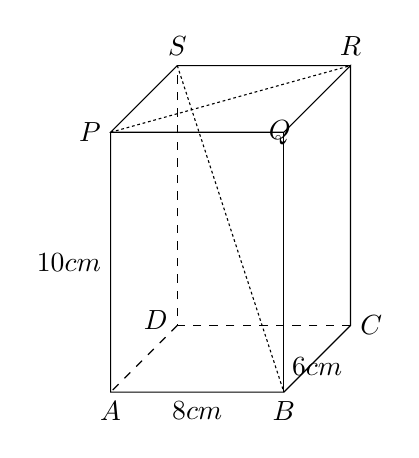
\begin{tikzpicture}[scale=1.1]
                      \draw (2,3,0) node [above] {$R$} --(0,3,0) node [above] {$S$} --(0,3,2) node [left] {$P$} --(2,3,2) node [above=6pt, left=-6pt] {$Q$} --(2,3,0)--(2,0,0) node [right] {$C$}--(2,0,2)node [below] {$B$} node [midway, right=12pt, below=-4pt] {$6cm$}--(0,0,2) node [below] {$A$} node [midway, below] {$8cm$} --(0,3,2) node [midway, left] {$10cm$};
                      \draw (2,3,2)--(2,0,2);
                      \draw[dashed](2,0,0)--(0,0,0)node [above=2pt, left] {$D$}--(0,3,0);
                      \draw[dashed](0,0,0)--(0,0,2);
                      \draw[dash pattern=on 1pt off 1pt] (0, 3, 2) -- (2,3,0);
                      \draw[dash pattern=on 1pt off 1pt] (0, 3, 0) -- (2,0,2);
                  \end{tikzpicture}
              \end{center}
        \item The diagram below shows a pyramid. Given that its base $PQRS$ is a square, $TR$
              is perpendicular to the base, $TS = 15cm$, $TR = 9cm$. Find:
              \begin{enumerate}
                  \item The length of $RS$.
                  \item The angle formed by line $PT$ and plane $PQRS$.
              \end{enumerate}
              \begin{center}
                  \tdplotsetmaincoords{70}{-20}
                  \begin{tikzpicture}[scale=0.7,tdplot_main_coords,line cap=butt,line join=bevel]
                      \draw (-2, 2, 0) node [left] {$S$} -- (-1,-3,0) node [below] {$P$} -- (3,-3,0) node [right] {$Q$};
                      \draw [dashed] (3, -3, 0) -- (2,2,0) node [below=8pt, left=-6pt] {$R$} -- (-2,2,0);
                      \draw [dashed] (2,2,0) -- (2,2,2.5) node [above] {$T$}  node [midway, right=12pt, below=4pt] {$9cm$};
                      \draw (-1,-3,0) -- (2,2,2.5) -- (3,-3,0);
                      \draw (2,2,2.5) -- (-2,2,0) node [midway, above left] {$15cm$};
                      \draw (1.71, 2, 0) -- (2, 2.8, 0) -- (2, 2, 0.32);
                  \end{tikzpicture}
              \end{center}
        \item The diagram below shows a right pyramid with height of $8cm$, its base is a
              rectangle, $E$ is the foot point from $V$ to the base. Given that $CD = 5cm$,
              $BC = 6cm$. Find:
              \begin{enumerate}
                  \item The angle formed by line $VA$ and line $VE$.
                  \item The angle formed by line $VC$ and plane $ABCD$.
              \end{enumerate}
              \begin{center}
                  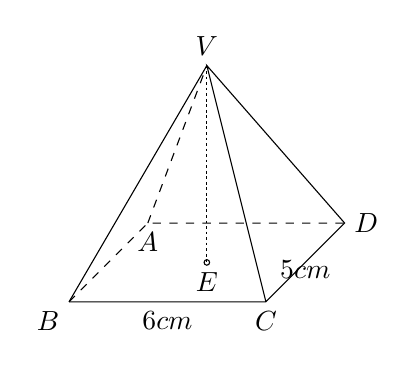
\begin{tikzpicture}
                      \tikzstyle{point}=[circle,thick,draw=black,fill=black,inner sep=0pt,minimum width=4pt,minimum height=4pt]
                      \node (a) at (0,0) {};
                      \node (b) at (2.5,0) {};
                      \node (c) at (3.5,1) {};
                      \node (d) at (1,1) {};
                      \node (e) at (1.75,3) {};
                      \draw (a.center) node [below left] {$B$} -- (b.center) node [below] {$C$} node [midway, below] {$6cm$} -- (c.center) node [ right] {$D$} node [midway, right=12pt, below=-4pt] {$5cm$} -- (e.center) node [above] {$V$} -- (b.center);
                      \draw (a.center) -- (e.center);
                      \draw[dashed] (a.center) -- (d.center) -- (c.center);
                      \draw[dashed] (d.center) node [below] {$A$} -- (e.center);
                      \node (f) at (1.75, 0.5) {};
                      \draw (f.center) circle (1pt);
                      \draw[dash pattern=on 1pt off 1pt] (e.center) -- (f.center) node [below] {$E$};
                  \end{tikzpicture}
              \end{center}
        \item The diagram below shows a right pyramid, its base $PQRS$ is a regtangle. Given
              that $SR = 6cm$, $QR = 8cm$, $VS = 13cm$. Find:
              \begin{enumerate}
                  \item The length of $PR$.
                  \item The height of the pyramid.
                  \item The angle of the line $VP$ and plane $PQRS$.
              \end{enumerate}
              \begin{center}
                  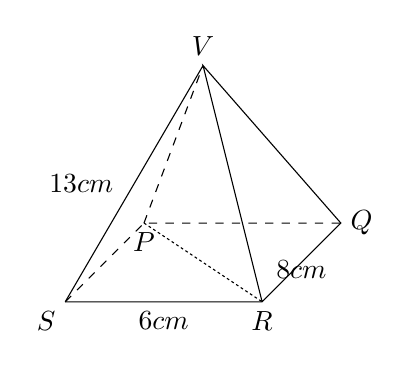
\begin{tikzpicture}
                      \tikzstyle{point}=[circle,thick,draw=black,fill=black,inner sep=0pt,minimum width=4pt,minimum height=4pt]
                      \node (a) at (0,0) {};
                      \node (b) at (2.5,0) {};
                      \node (c) at (3.5,1) {};
                      \node (d) at (1,1) {};
                      \node (e) at (1.75,3) {};
                      \draw (a.center) node [below left] {$S$} -- (b.center) node [below] {$R$} node [midway, below] {$6cm$} -- (c.center) node [ right] {$Q$} node [midway, right=12pt, below=-4pt] {$8cm$} -- (e.center) node [above] {$V$} -- (b.center);
                      \draw (a.center) -- (e.center) node [midway, left=4pt] {$13cm$};
                      \draw[dashed] (a.center) -- (d.center) -- (c.center);
                      \draw[dashed] (d.center) node [below] {$P$} -- (e.center);
                      \draw[dash pattern=on 1pt off 1pt] (d.center) -- (b.center);
                  \end{tikzpicture}
              \end{center}
        \item The diagram below shows a regular pyramid, the length of its lateral edge is
              $12cm$, its base $ABCD$ is a square with side length of $8cm$, $M$ is the
              midpoint of $BC$. Find:
              \begin{enumerate}
                  \item The angle formed by the lateral edge and the base of the pyramid.
                  \item The angle formed by line $VM$ and the base of the pyramid.
              \end{enumerate}
              \begin{center}
                  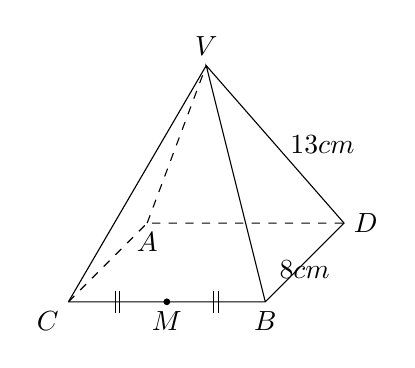
\begin{tikzpicture}
                      \tikzstyle{point}=[circle,thick,draw=black,fill=black,inner sep=0pt,minimum width=4pt,minimum height=4pt]
                      \node (a) at (0,0) {};
                      \node (b) at (2.5,0) {};
                      \node (c) at (3.5,1) {};
                      \node (d) at (1,1) {};
                      \node (e) at (1.75,3) {};
                      \draw (a.center) node [below left] {$C$} -- (b.center) node [below] {$B$} -- (c.center) node [right] {$D$} node [midway, right=12pt, below=-4pt] {$8cm$} -- (e.center) node [above] {$V$} node [midway, right=2pt] {$13cm$} -- (b.center);
                      \draw (a.center) -- (e.center);
                      \draw[dashed] (a.center) -- (d.center) -- (c.center);
                      \draw[dashed] (d.center) node [below] {$A$} -- (e.center);
                      \coordinate (m) at ($(a.center)!0.5!(b.center)$);
                      \filldraw (m) circle (1pt);
                      \node [below] at (m) {$M$};
                      \tkzMarkSegment[pos=.5,mark=||](a.center,m);
                      \tkzMarkSegment[pos=.5,mark=||](b.center,m);
                  \end{tikzpicture}
              \end{center}
        \item In the pyramid shown below, $\Delta ABC$ is a right-angled triangle, $CD$ is
              perpendicular to plane $ABC$, $CE$ is perpendicular to $AB$. Given that $AC =
                  15cm$, $BC = 20cm$ and $CD = 9cm$. Find:
              \begin{enumerate}
                  \item The length of $CE$.
                  \item $\angle CDE$.
                  \item The angle formed by line $AD$ and plane $ABC$.
              \end{enumerate}
              \begin{center}
                  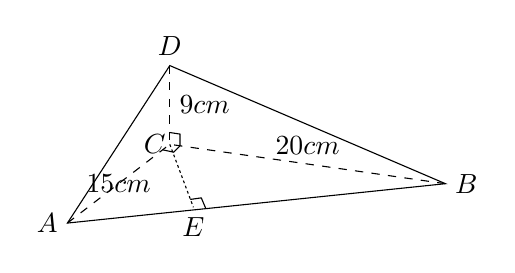
\begin{tikzpicture}
                      \draw (0.2, 0) node [left] {$A$} -- (1.5,2) node [above] {$D$} -- (5, 0.5) node [right] {$B$} -- cycle;
                      \draw [dashed] (0.2, 0) -- (1.5, 1) node [above=4pt, left=-2pt] {$C$} node [midway] {$15cm$};
                      \draw [dashed] (1.5, 2) -- (1.5, 1) node [midway, right] {$9cm$};
                      \draw [dashed] (5, 0.5) -- (1.5, 1)  node [midway, above] {$20cm$};
                      \draw[dash pattern=on 1pt off 1pt] (1.5, 1) -- (1.8, 0.2) node [below] {$E$};
                      \draw (1.5, 1.15) -- (1.63, 1.13) -- (1.63, 0.98) -- (1.55, 0.9) -- (1.41, 0.93);
                      \draw (1.76, 0.3) -- (1.9, 0.32) -- (1.955, 0.19);
                  \end{tikzpicture}
              \end{center}
        \item The diagram below shows a right prism, its base $CDF$ is a right-angled
              triangle. Given that $BC = 16.5cm$ and $AB = 12cm$. Assume that $CF = 2DF$,
              find:
              \begin{enumerate}
                  \item The angle formed by line $AB$ and plane $BCFE$.
                  \item The angle formed by line $AC$ and plan $BCFE$.
              \end{enumerate}
              \begin{center}
                  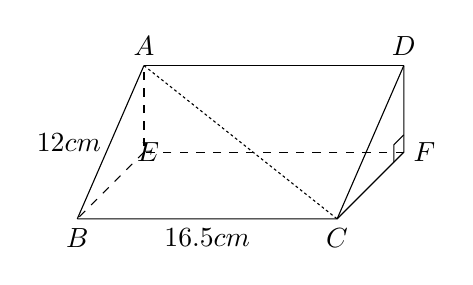
\begin{tikzpicture}[scale=1.1]
                      \draw (3,1,0) node [above] {$D$} --(0,1,0) node [above] {$A$};
                      \draw (3, 1, 0)--(3,0,0) node [right] {$F$} --(3,0,2)node [below] {$C$}--(0,0,2) node [below] {$B$} node [midway, below] {$16.5cm$};
                      \draw (0,1,0) -- (0,0,2) node [midway, left] {$12cm$};
                      \draw (3,1,0) -- (3,0,2);
                      \draw (3, 0.2, 0) -- (3, 0.2, 0.3) -- (3, 0.0, 0.3);
                      \draw[dashed](3,0,0)--(0,0,0) node [below=6pt, right=-6pt] {$E$}--(0,1,0);
                      \draw[dashed](0,0,0)--(0,0,2);
                      \draw[dash pattern=on 1pt off 1pt] (0, 1, 0) -- (3,0,2);
                  \end{tikzpicture}
              \end{center}
        \item The diagram below shows a cuboid with volume of $300cm^3$. Given that $AD =
                  2DC$ and $DN = 9cm$. Find the angle formed by line $AM$ and plane $KLMN$.
              \begin{center}
                  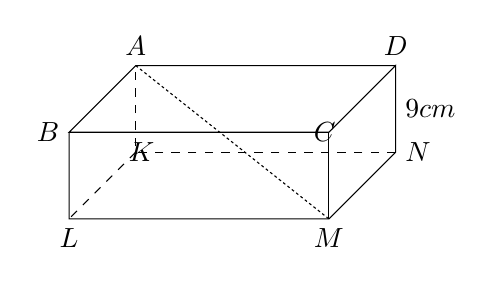
\begin{tikzpicture}[scale=1.1]
                      \draw (3,1,0) node [above] {$D$} --(0,1,0) node [above] {$A$} --(0,1,2) node [left] {$B$} --(3,1,2) node [above=6pt, left=-6pt] {$C$} --(3,1,0)--(3,0,0) node [right] {$N$} node [midway, right] {$9cm$}--(3,0,2)node [below] {$M$}--(0,0,2) node [below] {$L$} --(0,1,2);
                      \draw (3,1,2)--(3,0,2);
                      \draw[dashed](3,0,0)--(0,0,0) node [below=6pt, right=-6pt] {$K$}--(0,1,0);
                      \draw[dashed](0,0,0)--(0,0,2);
                      \draw[dash pattern=on 1pt off 1pt] (0, 1, 0) -- (3,0,2);
                  \end{tikzpicture}
              \end{center}
        \item The diagram below shows a cuboid. Given that $AB = 13cm$, $BC = 6cm$, $CG =
                  4cm$. M is a point on $AB$, $AM = 9cm$. Find:
              \begin{enumerate}
                  \item The angle formed by line $HM$ and plane $ABCG$.
                  \item The angle formed by line $HM$ and plane $HDAE$.
                  \item The angle formed by line $AG$ and plane $CDHG$.
              \end{enumerate}
              \begin{center}
                  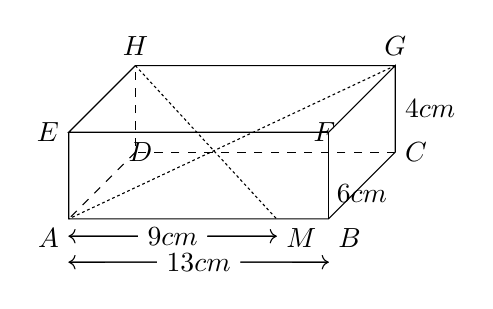
\begin{tikzpicture}[scale=1.1]
                      \draw (3,1,0) node [above] {$G$} --(0,1,0) node [above] {$H$} --(0,1,2) node [left] {$E$} --(3,1,2) node [above=6pt, left=-6pt] {$F$} --(3,1,0)--(3,0,0) node [right] {$C$} node [midway, right] {$4cm$}--(3,0,2)node [below right] {$B$} node [midway, right=16pt, below=-4pt] {$6cm$}--(0,0,2) node [below left] {$A$} --(0,1,2);
                      \draw (3,1,2)--(3,0,2);
                      \draw[dashed](3,0,0)--(0,0,0) node [below=6pt, right=-6pt] {$D$}--(0,1,0);
                      \draw[dashed](0,0,0)--(0,0,2);
                      \draw[dash pattern=on 1pt off 1pt] (0, 1, 0) -- (2.4,0,2) node [below right] {$M$};
                      \draw[dash pattern=on 1pt off 1pt] (3, 1, 0) -- (0, 0, 2);
                      \path (0, -0.2, 2) -- node (success) {$9cm$} (2.4, -0.2, 2);
                      \draw[->] (0, -0.2, 2) -- (success) -- (2.4, -0.2, 2);
                      \draw[->] (2.4, -0.2, 2) -- (success) -- (0, -0.2, 2);
                      \path (0, -0.5, 2) -- node (success) {$13cm$} (3, -0.5, 2);
                      \draw[->] (0, -0.5, 2) -- (success) -- (3, -0.5, 2);
                      \draw[->] (3, -0.5, 2) -- (success) -- (0, -0.5, 2);
                  \end{tikzpicture}
              \end{center}
        \item The diagram below shows a regular prism, its bases $ADS$ and $BCR$ are
              equiliteral triangles. Given that $AB = 16cm$, $BC = 7cm$, $SP = 5cm$. Find:
              \begin{enumerate}
                  \item The length of $BP$.
                  \item The angle formed by line $BP$ and plane $ABCD$.
              \end{enumerate}
              \begin{center}
                  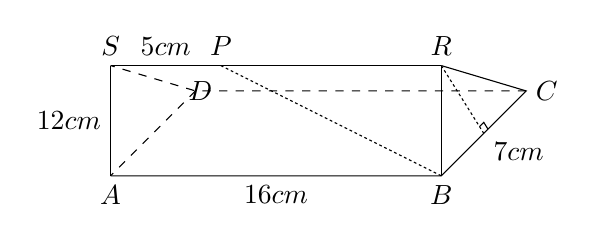
\begin{tikzpicture}[scale=1.4]
                      \draw (3,1,2) node [above] {$R$} --(0,1,2) node [above] {$S$};
                      \draw (3, 1, 2)--(3,0,0) node [right] {$C$} --(3,0,2)node [below] {$B$} node [midway, below right] {$7cm$} --(0,0,2) node [below] {$A$} node [midway, below] {$16cm$};
                      \draw (0,1,2) -- (0,0,2) node [midway, left] {$12cm$};
                      \draw (3,1,2) -- (3,0,2);
                      \draw[dashed](3,0,0)--(0,0,0) node [below=6pt, right=-6pt] {$D$}--(0,1,2);
                      \draw[dashed](0,0,0)--(0,0,2);
                      \draw[dash pattern=on 1pt off 1pt] (1, 1, 2) node [above] {$P$} -- (3,0,2);
                      \draw (0, 1, 2) -- (1, 1, 2) node [midway, above] {$5cm$};
                      \draw[dash pattern=on 1pt off 1pt] (3, 1, 2) -- (3, 0, 1);
                      \draw (3, 0.1, 1.1) -- (3, 0.1, 1) -- (3, 0, 0.9);
                  \end{tikzpicture}
              \end{center}
        \item The diagram below shows a roof, $HK$ is the ridge of the roof, its edges $HA$,
              $HD$, $KB$, $KC$ are euqal in length. Both of the planes $HAD$ and $KBC$ form a
              $44^o$ angle with plane $ABCD$. Given that $S$ and $T$ are the midpoints of
              $BC$ and $AD$ respectively. Find:
              \begin{enumerate}
                  \item The distance from line $HK$ to plane $ABCD$.
                  \item The length of $HK$.
                  \item The angle formed by line $HA$ and plane $ABCD$.
              \end{enumerate}
              \begin{center}
                  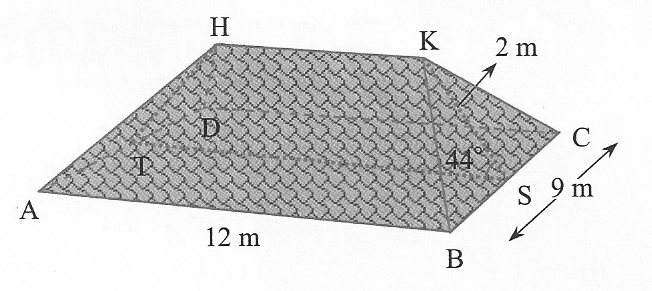
\includegraphics[scale=0.9]{roof}
              \end{center}
        \item The length, width and height of a hall are $20m$, $15m$, and $4m$ respectively.
              Find:
              \begin{enumerate}
                  \item The length of the diagonal of the hall.
                  \item The angle formed by the diagonal and the floor of the hall.
              \end{enumerate}
              \begin{center}
                  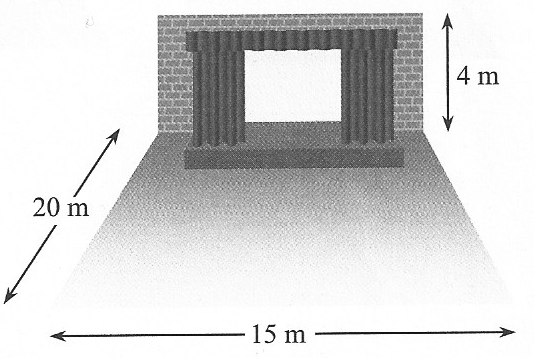
\includegraphics[scale=0.9]{hall}
              \end{center}
        \item In the diagram below, $ABCD$ represents a rectangular plank with length and
              width of $60cm$ and $36cm$ respectively, its base $BC$ is on the ground and the
              top of it lies on the wall. Assume that the distance between $BC$ and the
              corner of the wall is $12cm$, find the angle formed by the diagonal $BD$ of the
              plank and the ground.
              \begin{center}
                  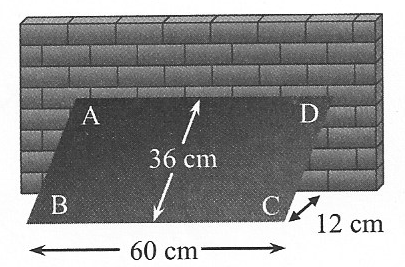
\includegraphics[scale=0.9]{wall}
              \end{center}
    \end{enumerate}

    \section{Angle Formed by Two Planes}

    There are three types positional relationship between two planes:

    \begin{enumerate}
        \item Two planes coincide with each other.
              \begin{center}
                  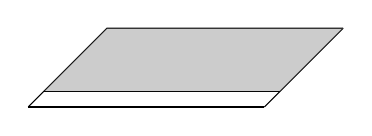
\begin{tikzpicture}
                      \draw (0,0)--(3,0);
                      \draw (3,0)--(4,1);
                      \draw (4,1)--(1,1)--(0,0);
                      \draw (0.2, 0.2) -- (3.2, 0.2);
                      \fill [color=gray,opacity=0.4] (0.2, 0.2) -- (3.2, 0.2) -- (4, 1) -- (1, 1) -- cycle;
                  \end{tikzpicture}
              \end{center}
        \item Two planes intersect with each other at a line.
              \begin{center}
                  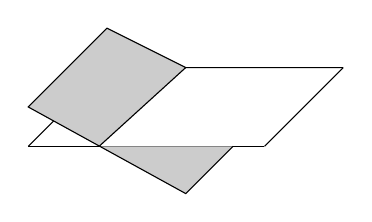
\begin{tikzpicture}
                      \draw (0,0)--(3,0);
                      \draw (3,0)--(4,1);
                      \draw (4,1)--(1,1)--(0,0);
                      \filldraw [fill=gray!40] (0.9, 0) -- (2,1) -- (1, 1.5) -- (0, 0.5) -- (2, -0.6) -- (2.6, 0);
                  \end{tikzpicture}
              \end{center}
        \item Two planes are parallel to each other and do not intersect with each other.
              \begin{center}
                  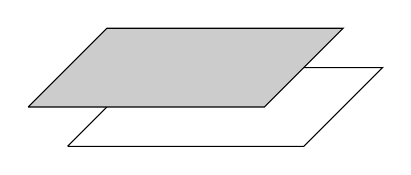
\begin{tikzpicture}
                      \draw (0,0)--(3,0)--(4,1)--(1,1)--(0,0);
                      \filldraw [fill=gray!40] (-0.5,0.5)--(2.5,0.5)--(3.5,1.5)--(0.5,1.5)--(-0.5,0.5);
                  \end{tikzpicture}
              \end{center}
    \end{enumerate}

    Two non-parallel planes intersect with each other at a line, the line is called
    the \emph{common edge}. At any point on the common edge, draw a line
    perpendicular to the common edge on each plane, the acute angles formed by
    these two perpendicular lines are called \emph{the angle formed by the two
        planes}.
    \begin{center}
        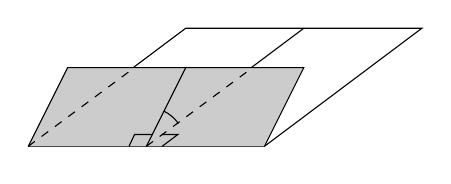
\begin{tikzpicture}
            \draw (0,0)--(3,0)--(5,1.5)--(2,1.5)--(0,0);
            \draw (1.5, 0) -- (3.5, 1.5);
            \filldraw[fill=gray!40] (0, 0) -- (0.5, 1) -- (3.5, 1) -- (3, 0);
            \draw (1.5, 0) -- (2, 1);
            \draw [dashed] (1.5, 0) -- (2.85, 1);
            \draw [dashed] (0, 0) -- (1.35, 1);
            \draw (1.28, 0) -- (1.35, 0.15) -- (1.58, 0.15);
            \draw (1.7, 0.15) -- (1.9, 0.15) -- (1.7, 0);
            \node (O) at (1.5, 0) {};
            \node (x) at (2, 1) {};
            \node (z) at (2.9, 1) {};
            \pic [draw,
                angle radius=5mm, angle eccentricity=0.1] {angle = z--O--x};
        \end{tikzpicture}
    \end{center}

    \subsection{Practice 2}

    \begin{enumerate}
        \item The diagram below shows a cuboid with length of $12cm$, width of $10cm$ and
              height of $6cm$.
              \begin{enumerate}
                  \item Find the angle formed by plane $EBCH$ and plane $ABCD$.
                  \item Assume that $M$ is a point on $HG$, find the angle formed by plane $MAB$ and
                        plane $ABCD$.
              \end{enumerate}
              \begin{center}
                  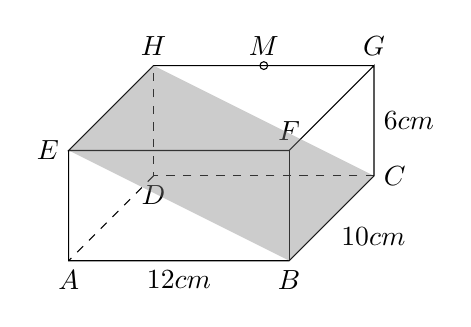
\begin{tikzpicture}[scale=1.4]
                      \draw (2,1,0) node [above] {$G$} --(0,1,0) node [above] {$H$} --(0,1,2) node [left] {$E$} --(2,1,2)node [above] {$F$} --(2,1,0) --(2,0,0) node [right] {$C$} node [midway, right] {$6cm$} --(2,0,2) node [below] {$B$}  node [midway, below right] {$10cm$} --(0,0,2) node [below] {$A$}  node [midway, below] {$12cm$} --(0,1,2);
                      \draw (2,1,2)--(2,0,2);
                      \draw[dashed](2,0,0)--(0,0,0) node [below] {$D$}--(0,1,0);
                      \draw[dashed](0,0,0)--(0,0,2);
                      \fill [color=gray, opacity=0.4] (0, 1, 0) -- (0, 1, 2) -- (2, 0, 2) -- (2, 0, 0) -- cycle;
                      \draw (1,1,0) circle (1pt) node [above] {$M$};
                  \end{tikzpicture}
              \end{center}

        \item The diagram below shows a regular prism, its bases $ABC$ and $DEF$ are
              equilateral triangles with side length of $5cm$. Given that the height of the
              prism is $10cm$, find:
              \begin{enumerate}
                  \item The length of $BF$.
                  \item The angle formed by plane $ABF$ and plane $ABC$.
              \end{enumerate}
              \begin{center}
                  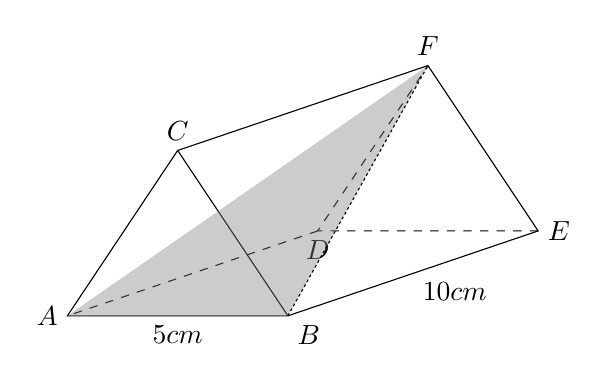
\begin{tikzpicture}[scale=1.4]
                      \draw (1,1.5,2) node [above] {$C$} --(2.5,1.5,0) --(3.5,0,0) node [right] {$E$} --(2,0,2) node [below right] {$B$}  node [midway, below right] {$10cm$} --(0,0,2) node [left] {$A$}  node [midway, below] {$5cm$} --(1,1.5,2);
                      \draw (1,1.5,2)--(2,0,2);
                      \draw[dashed](3.5,0,0)--(1.5,0,0) node [below] {$D$}--(2.5,1.5,0) node [above] {$F$};
                      \draw[dashed](1.5,0,0)--(0,0,2);
                      \fill[color=gray, opacity=0.4] (2.5, 1.5, 0) -- (0, 0, 2) -- (2, 0, 2);
                      \draw [dash pattern=on 1pt off 1pt] (2, 0, 2) -- (2.5, 1.5, 0);
                  \end{tikzpicture}
              \end{center}
    \end{enumerate}

    \subsection{Exercise 17.3}

    \begin{enumerate}
        \item The diagram below shows a cuboid with length of $8cm$, width of $6cm$ and
              height of $4cm$. Find the angle formed by plane $ABMN$ and $KLMN$.
              \begin{center}
                  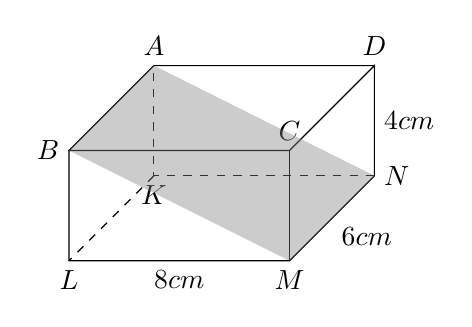
\begin{tikzpicture}[scale=1.4]
                      \draw (2,1,0) node [above] {$D$} --(0,1,0) node [above] {$A$} --(0,1,2) node [left] {$B$} --(2,1,2)node [above] {$C$} --(2,1,0) --(2,0,0) node [right] {$N$} node [midway, right] {$4cm$} --(2,0,2) node [below] {$M$}  node [midway, below right] {$6cm$} --(0,0,2) node [below] {$L$} node [midway, below] {$8cm$} --(0,1,2);
                      \draw (2,1,2)--(2,0,2);
                      \draw[dashed](2,0,0)--(0,0,0) node [below] {$K$}--(0,1,0);
                      \draw[dashed](0,0,0)--(0,0,2);
                      \fill [color=gray, opacity=0.4] (0, 1, 0) -- (0, 1, 2) -- (2, 0, 2) -- (2, 0, 0) -- cycle;
                  \end{tikzpicture}
              \end{center}
        \item In the right prism shown below, $ABCD$ is a rectangle with length of $20cm$ and
              width of $12cm$, $BCRQ$ is a trapezoid, $\angle QBC$ and $\angle RCB$ are both
              right angles, $BQ = 5cm$, $CR = 10cm$. Find the angle formed by plane $PQRS$
              and plane $ABCD$.
              \begin{center}
                  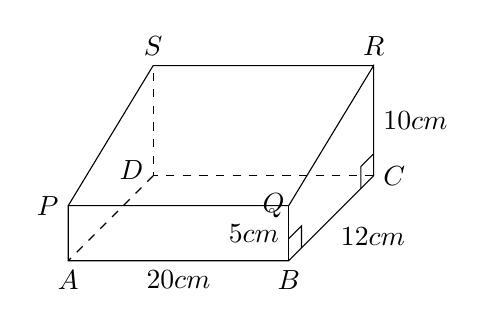
\begin{tikzpicture}[scale=1.4]
                      \draw (2,1,0) node [above] {$R$} --(0,1,0) node [above] {$S$} --(0,0.5,2) node [left] {$P$} --(2,0.5,2)node [above=6pt,left=-2pt] {$Q$} --(2,1,0) --(2,0,0) node [right] {$C$} node [midway, right] {$10cm$} --(2,0,2) node [below] {$B$}  node [midway, below right] {$12cm$} --(0,0,2) node [below] {$A$} node [midway, below] {$20cm$} --(0,0.5,2);
                      \draw (2,0.5,2)--(2,0,2) node [midway, left] {$5cm$};
                      \draw[dashed](2,0,0)--(0,0,0) node [above = 2pt, left] {$D$}--(0,1,0);
                      \draw[dashed](0,0,0)--(0,0,2);
                      \draw (2, 0.2, 0) -- (2, 0.2, 0.3) -- (2, 0.0, 0.3);
                      \draw (2, 0.2, 2) -- (2, 0.2, 1.7) -- (2, 0.0, 1.7);
                  \end{tikzpicture}
              \end{center}
        \item The diagram below shows a cuboid, $AB = 8cm$, $BC = 6cm$, $CT = 5cm$, $X$ is
              the midpoint of $TU$. Find:
              \begin{enumerate}
                  \item The angle formed by plane $XAB$ and plane $ABCD$.
                  \item The angle formed by plane $BCUR$ and plane $ADUR$.
                  \item The angle formed by plane $ABTU$ and plane $ABCD$.
              \end{enumerate}
              \begin{center}
                  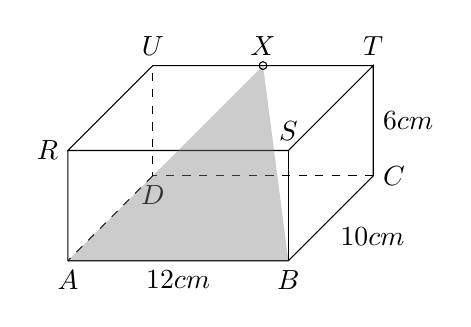
\begin{tikzpicture}[scale=1.4]
                      \draw (2,1,0) node [above] {$T$} --(0,1,0) node [above] {$U$} --(0,1,2) node [left] {$R$} --(2,1,2)node [above] {$S$} --(2,1,0) --(2,0,0) node [right] {$C$} node [midway, right] {$6cm$} --(2,0,2) node [below] {$B$}  node [midway, below right] {$10cm$} --(0,0,2) node [below] {$A$}  node [midway, below] {$12cm$} --(0,1,2);
                      \draw (2,1,2)--(2,0,2);
                      \draw[dashed](2,0,0)--(0,0,0) node [below] {$D$}--(0,1,0);
                      \draw[dashed](0,0,0)--(0,0,2);
                      \fill [color=gray, opacity=0.4] (2, 0, 2) -- (0, 0, 2) -- (1,1,0) -- cycle;
                      \draw (1,1,0) circle (1pt) node [above] {$X$};
                  \end{tikzpicture}
              \end{center}
        \item The diagram below shows a right pyramid, its bases $ABE$ and $DCF$ are
              right-angled triangles. Given that $AE = 4cm$, $BE = \frac{2}{3}EF$, $EF =
                  4DF$, find the angle formed by plane $ABCD$ and plane $BCFE$.
              \begin{center}
                  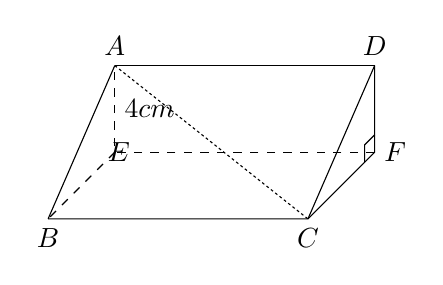
\begin{tikzpicture}[scale=1.1]
                      \draw (3,1,0) node [above] {$D$} --(0,1,0) node [above] {$A$};
                      \draw (3, 1, 0)--(3,0,0) node [right] {$F$} --(3,0,2)node [below] {$C$}--(0,0,2) node [below] {$B$};
                      \draw (0,1,0) -- (0,0,2);
                      \draw (3,1,0) -- (3,0,2);
                      \draw (3, 0.2, 0) -- (3, 0.2, 0.3) -- (3, 0.0, 0.3);
                      \draw[dashed](3,0,0)--(0,0,0) node [below=6pt, right=-6pt] {$E$}--(0,1,0)  node [midway,right] {$4cm$};
                      \draw[dashed](0,0,0)--(0,0,2);
                      \draw[dash pattern=on 1pt off 1pt] (0, 1, 0) -- (3,0,2);
                  \end{tikzpicture}
              \end{center}
        \item In the pyramid shown below, $PQT$, $SPT$, and $SRT$ are all right-angled
              triangles, $PQRS$ is a triangle. Given that $PQ = 5cm$, $RT = 13cm$, $PT =
                  20cm$. Find:
              \begin{enumerate}
                  \item The height of the prism.
                  \item The angle formed by line $TQ$ and plane $QST$.
                  \item The angle formed by plane $RST$ and $PQT$.
              \end{enumerate}
              \begin{center}
                  \tdplotsetmaincoords{70}{-20}
                  \begin{tikzpicture}[scale=0.7,tdplot_main_coords,line cap=butt,line join=bevel]
                      \draw (-2, 2, 0) node [left] {$P$} -- (-1,-0.5,0) node [below] {$Q$} node [midway, left=8pt,below=-2pt] {$5cm$} -- (3,-0.5,0) node [right] {$R$};
                      \draw [dashed] (3, -0.5, 0) -- (2,2,0) node [below=8pt, left=-6pt] {$S$} -- (-2,2,0);
                      \draw [dashed] (2,2,0) -- (2,2,5) node [above] {$T$};
                      \draw (-1,-0.5,0) -- (2,2,5) -- (3,-0.5,0) node [midway, right] {$13cm$};
                      \draw (2,2,5) -- (-2,2,0) node [midway, above left] {$20cm$};
                      \draw (1.71, 2, 0) -- (2, 2.8, 0) -- (2, 2, 0.32) -- (2, 1.2, 0.5) -- (2, 1.2, 0.15);
                      \draw (-1.95, 1.6, 0.4) -- (-1.9, 0.9, 0.5) -- (-2.05, 1, 0.25);
                  \end{tikzpicture}
              \end{center}
        \item The diagram below shows a right prism, its base $BCGF$ is a trapezoid, $BC = BF
                  = 12cm$, $FG = 16cm$. The lateral face $EFGH$ is a square, and is
              perependicular to another lateral face $ABFE$. Find:
              \begin{enumerate}
                  \item The angle formed by plane $CDHG$ and plane $EFGH$.
                  \item The angle formed by plane $ABH$ and plane $ABFE$.
              \end{enumerate}
              \begin{center}
                  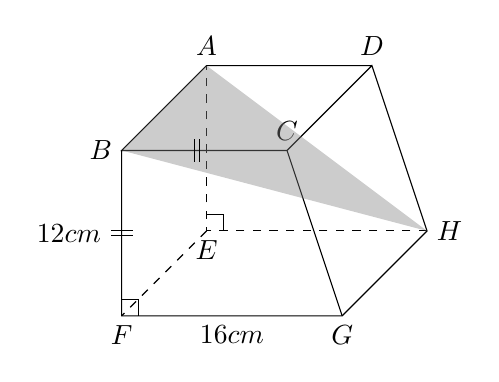
\begin{tikzpicture}[scale=1.4]
                      \draw (1.5,1.5,0) node [above] {$D$} --(0,1.5,0) node [above] {$A$} --(0,1.5,2) node [left] {$B$} --(1.5,1.5,2)node [above] {$C$} --(1.5,1.5,0) --(2,0,0) node [right] {$H$} --(2,0,2) node [below] {$G$} --(0,0,2) node [below] {$F$} node [midway, below] {$16cm$} --(0,1.5,2) node [midway, left=4pt] {$12cm$};
                      \draw (1.5,1.5,2)--(2,0,2);
                      \draw[dashed](2,0,0)--(0,0,0) node [below] {$E$}--(0,1.5,0);
                      \draw[dashed](0,0,0)--(0,0,2);
                      \fill [color=gray, opacity=0.4] (0, 1.5, 0) -- (0, 1.5, 2) -- (2, 0, 0) -- cycle;
                      \node (a) at (0,1.5,2) {};
                      \node (b) at (1.5,1.5,2) {};
                      \node (c) at (0,0,2) {};
                      \tkzMarkSegment[pos=.45,mark=||](a,b);
                      \tkzMarkSegment[pos=.5,mark=||](a,c);
                      \draw (0, 0.15, 0) -- (0.15, 0.15, 0) -- (0.15, 0, 0);
                      \draw (0, 0.15, 2) -- (0.15, 0.15, 2) -- (0.15, 0, 2);
                  \end{tikzpicture}
              \end{center}
        \item In the rectangle shown below, $BC = 8cm$, $CD = 6cm$, $BQ = 10cm$. Given that
              $M$ is the midpoint of $PQ$. Find:
              \begin{enumerate}
                  \item The angle formed by line $MD$ and plane $PQBA$.
                  \item The angle formed by plane $AMD$ and plane $ABCD$.
              \end{enumerate}
              \begin{center}
                  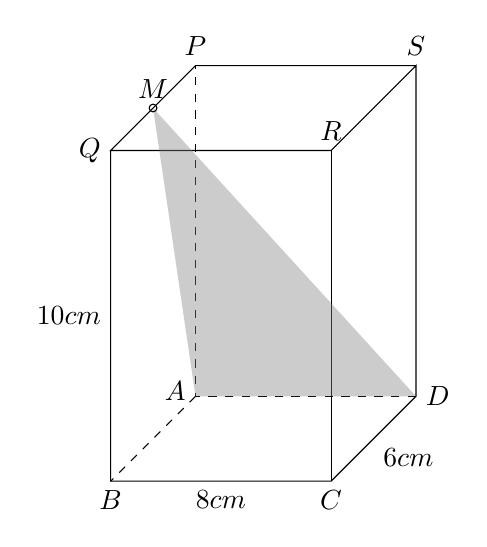
\begin{tikzpicture}[scale=1.4]
                      \draw (2,3,0) node [above] {$S$} --(0,3,0) node [above] {$P$} --(0,3,2) node [left] {$Q$} --(2,3,2)node [above] {$R$} --(2,3,0) --(2,0,0) node [right] {$D$} --(2,0,2) node [below] {$C$}  node [midway, below right] {$6cm$} --(0,0,2) node [below] {$B$}  node [midway, below] {$8cm$} --(0,3,2) node [midway, left] {$10cm$};
                      \draw (2,3,2)--(2,0,2);
                      \draw[dashed](2,0,0)--(0,0,0) node [above=2pt, left] {$A$}--(0,3,0);
                      \draw[dashed](0,0,0)--(0,0,2);
                      \fill [color=gray, opacity=0.4] (0, 3, 1) -- (0,0,0) -- (2, 0, 0) -- cycle;
                      \draw (0,3,1) circle (1pt) node [above] {$M$};
                  \end{tikzpicture}
              \end{center}
        \item The diagram below shows a pyramid with an isoceles triangle base. Given that
              $CD = CE = 5cm$, $ED = 6cm$, $ACD$ is a right-angled triangle, $B$ is a point
              on $AC$, $AD = 2cm$, $BC = 4cm$. Find:
              \begin{enumerate}
                  \item The angle formed by plane $BDE$ and plane $CDE$.
                  \item The angle formed by the plane $ADE$ and $CDE$.
              \end{enumerate}
              \begin{center}
                  \tdplotsetmaincoords{70}{70}
                  \begin{tikzpicture}[scale=0.6,tdplot_main_coords,declare function={d=6;}]
                      \path (0,0,0)       coordinate (A) node [left] {$E$}
                      (d,0,0)        coordinate (C) node [below] {$D$}
                      (d/2,{d*sqrt(3)/2},0)    coordinate (B) node [right] {$C$}
                      (d/2,{d*sqrt(3)/2 - 0.15} ,d-1.5) coordinate (F) node [right] {$B$}
                      (d/2,d/2 + 2,{d/sqrt(2) + 2}) coordinate (D) node [above] {$A$}
                      ($ (A)!0.5!(C) $) coordinate (M);
                      \foreach \p/\g in {A/-90,B/-90,C/-90,D/90}
                      \path (\p)+(\g:3mm);
                      \draw (F) circle (1.2pt);
                      \draw (D) -- (A) (D) -- (B) (D) -- (C) (A) -- (C) -- (B);
                      \draw [dashed] (A) -- (B);
                      \path (D) -- (F) node [midway, right] {$2cm$};
                      \path (B) -- (F) node [midway, right] {$4cm$};
                      \path (C) -- (B) node [midway, right=12pt, below=4pt] {$5cm$};
                      \path (A) -- (C) node [midway, left=14pt, below=-4pt] {$6cm$};
                      \fill [color=gray, opacity=0.4] (A) -- (C) -- (F) -- cycle;
                      \draw (d/2,{d*sqrt(3)/2},0.5) -- (d/2,{d*sqrt(3)/2 - 0.4} ,0.4) -- (d/2,{d*sqrt(3)/2 - 0.4} ,-0.1);
                      \tkzMarkSegment[pos=.45,mark=||](A,B);
                      \tkzMarkSegment[pos=.45,mark=||](B,C);
                  \end{tikzpicture}
              \end{center}
        \item The diagram below shows a regular pyramid with a square base. Given that $PQ =
                  15cm$, $PV = 20cm$. Find:
              \begin{enumerate}
                  \item The angle formed by linee $PV$ and plane $PQRS$.
                  \item The angle formed by the lateral faces and the base of the pyramid.
              \end{enumerate}
              \begin{center}
                  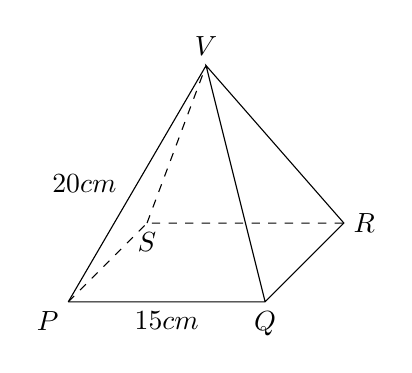
\begin{tikzpicture}
                      \tikzstyle{point}=[circle,thick,draw=black,fill=black,inner sep=0pt,minimum width=4pt,minimum height=4pt]
                      \node (a) at (0,0) {};
                      \node (b) at (2.5,0) {};
                      \node (c) at (3.5,1) {};
                      \node (d) at (1,1) {};
                      \node (e) at (1.75,3) {};
                      \draw (a.center) node [below left] {$P$} -- (b.center) node [below] {$Q$} node [midway, below] {$15cm$} -- (c.center) node [ right] {$R$} -- (e.center) node [above] {$V$} -- (b.center);
                      \draw (a.center) -- (e.center) node [midway, left=4pt] {$20cm$};
                      \draw[dashed] (a.center) -- (d.center) -- (c.center);
                      \draw[dashed] (d.center) node [below] {$S$} -- (e.center);
                  \end{tikzpicture}
              \end{center}
        \item The diagram below shows a right pyramid with lateral edges of $13cm$. Its base
              $ABCD$ is a rectangle with length of $12cm$ and width of $10cm$. Find:
              \begin{enumerate}
                  \item The angle formed by plane $VBC$ and plane $ABCD$.
                  \item The angle formed by plane $VCD$ and plane $ABCD$.
              \end{enumerate}
              \begin{center}
                  \begin{tikzpicture}
                      \tikzstyle{point}=[circle,thick,draw=black,fill=black,inner sep=0pt,minimum width=4pt,minimum height=4pt]
                      \node (a) at (0,0) {};
                      \node (b) at (2.5,0) {};
                      \node (c) at (3.5,1) {};
                      \node (d) at (1,1) {};
                      \node (e) at (1.75,3) {};
                      \draw (a.center) node [below left] {$A$} -- (b.center) node [below] {$B$} node [midway, below] {$12cm$} -- (c.center) node [ right] {$C$} node [midway, right=12pt, below=-4pt] {$10cm$} -- (e.center) node [above] {$V$} -- (b.center);
                      \draw (a.center) -- (e.center) node [midway, left=4pt] {$13cm$};
                      \draw[dashed] (a.center) -- (d.center) -- (c.center);
                      \draw[dashed] (d.center) node [below] {$D$} -- (e.center);
                  \end{tikzpicture}
              \end{center}
        \item The diagram below shows a right pyramid with lateral edges of $18cm$, its base
              $ABCD$ is a rectangle with length of $15cm$ and width of $10cm$. Find:
              \begin{enumerate}
                  \item The height of the pyramid.
                  \item The angle formed by plane $VAB$ and plane $ABCD$.
                  \item The angle formed by plane $VBC$ and plane $VAD$.
              \end{enumerate}
              \begin{center}
                  \begin{tikzpicture}
                      \tikzstyle{point}=[circle,thick,draw=black,fill=black,inner sep=0pt,minimum width=4pt,minimum height=4pt]
                      \node (a) at (0,0) {};
                      \node (b) at (2.5,0) {};
                      \node (c) at (3.5,1) {};
                      \node (d) at (1,1) {};
                      \node (e) at (1.75,3) {};
                      \draw (a.center) node [below left] {$A$} -- (b.center) node [below] {$B$} node [midway, below] {$15cm$} -- (c.center) node [ right] {$C$} node [midway, right=12pt, below=-4pt] {$10cm$} -- (e.center) node [above] {$V$} -- (b.center);
                      \draw (a.center) -- (e.center) node [midway, left=4pt] {$18cm$};
                      \draw[dashed] (a.center) -- (d.center) -- (c.center);
                      \draw[dashed] (d.center) node [below] {$D$} -- (e.center);
                  \end{tikzpicture}
              \end{center}
        \item The diagram below shows a right prism with isoceles triangle bases. The side
              length and base length of the triangle base are $10cm$ and $16cm$ respectively,
              the height of the prism is $20cm$. Given that $P$ is the midpoint of $AB$.
              Find:
              \begin{enumerate}
                  \item The length of $PC$.
                  \item The angle formed by line $EC$ and plane $ABCD$.
                  \item The angle formed by plane $DCE$ and plane $ABCD$.
              \end{enumerate}
              \begin{center}
                  \begin{tikzpicture}[scale=1.4]
                      \draw (1,1.5,2) node [above] {$E$} --(2.5,1.5,0) --(3.5,0,0) node [right] {$C$} node [midway, right] {$6cm$} --(2,0,2) node [below right] {$B$}  node [midway, below right] {$20cm$} --(0,0,2) node [left] {$A$}  --(1,1.5,2) node [midway, left=4pt] {$10cm$};
                      \draw (1,1.5,2)--(2,0,2);
                      \draw[dashed](3.5,0,0)--(1.5,0,0) node [below] {$D$}--(2.5,1.5,0) node [above] {$F$};
                      \draw[dashed](1.5,0,0)--(0,0,2);
                      \fill[color=gray, opacity=0.4] (1, 1.5, 2) -- (3.5, 0, 0) -- (1.5, 0, 0);
                      \draw (0, -1, -0.6) circle (1pt);
                      \draw [dash pattern=on 1pt off 1pt] (0, -1, -0.6) -- (3.5, 0, 0);
                      \path (0, -0.2, 2) -- node (success) {$16cm$} (2, -0.2, 2);
                      \draw[->] (0, -0.2, 2) -- (success) -- (2, -0.2, 2);
                      \draw[->] (2, -0.2, 2) -- (success) -- (0, -0.2, 2);
                      \node (a) at (1,1.5,2) {};
                      \node (b) at (2, 0, 2) {};
                      \node (c) at (0,0,2) {};
                      \node (d) at (1.5, 0, 0) {};
                      \node (e) at (2.5, 1.5, 0) {};
                      \node (f) at (3.5, 0, 0) {};
                      \tkzMarkSegment[pos=.45,mark=||](a,b);
                      \tkzMarkSegment[pos=.5,mark=||](a,c);
                      \tkzMarkSegment[pos=0.5,mark=||](e,f);
                      \tkzMarkSegment[pos=0.5,mark=||](e,d);
                  \end{tikzpicture}
              \end{center}

    \end{enumerate}

\end{multicols}
\end{document}